This section presents simulation results that show how the  the planned impulses and the pattern of retraction force, 
obtained running  the optimization of Section \ref{sec:motionP}, are able to bring the robot to a desired target. 
The OCP solver used is PINS~\cite{pins:1,pins:2,pins:3}, which uses the indirect approach based on the Pontryagin Maximum Principle.

% 1st experiment: validation of optimization with 2 models, with obstacle
In a first experiment, we run the optimization to perform  a 12 $m$ jump starting from an initial 
position $p_0 = \mat{0.024& 0& -8}^T$ up to a target at $p_f = \mat{3 & 3 &-20}^T$ $[m]$. As additional constraint,
during the jump, the robot has to avoid a rock pillar that is laying  the wall, that we model as a 20 $m$ high cone with a base of radius 2.5 $m$.
We validate the result of the optimization in the case of the simplified model (in a Matlab environment)
and for the full 3D model. In this case we built a Gazebo simulator based on the URDF  description \cite{urdf} of the robot.
The physical parameters of the robot and of the environment together with the 
optimization settings, are reported in Table \ref{tab:params}:
%
\begin{table}[!tbp]
	\centering
	\caption{ Simulations parameters}
		\begin{tabular}{l c c  } \hline\hline
			\textbf{Name} \quad                  & \textbf{Symbol}                     & \textbf{Value}  \\ \hline
					Robot mass                   & m  & 5                 \\ 
					Max. impulse  [N]       	 & $F_{u}^{\text{max}}$				& 1000   \\
					Max. retraction force [N]    & $F_r^{\text{max}} $			& 200    \\
					Friction coeff.				 & $ \mu $ 					        & 0.87   \\
					Thrust impulse duration	[s]  & 	$T_{th}$  				& 0.025\\
					Discretization steps         & N 						& 20\\					        
			\hline\hline 					    					    					    
		\end{tabular}
		\label{tab:params}
\end{table}
%
For the Matlab simulation we simply integrate equation \eqref{eq:nonlinearDyn} 
with a ode45 Runge Kutta variable-step integration scheme.
For the Gazebo simulation, we assume to apply the push impulse as a force $F_c$ at the contact point.
Therefore we employ the leg dynamics to define the mapping between the contact force $F_c$ and the torques $\tau_{\text{leg}}$ at the leg joints:
%
\begin{equation}
\tau_{\text{leg}}^d= \mat{\tau_{HP} \\ \tau_{HR} \\ f_{K}} =  h_{\text{leg}} -J_{\text{leg}}^T \underbrace{\left(R_e^\mathcal{W}  \mat{F_{u,n} \\ F_{u,t} \\ 0} \right) 	}_{F_c}
\end{equation}
%
Where $J_{\text{leg}} \in \Rnum^{3 \times 3}$ is the sub-matrix of the Jacobian $J$ relative to the leg jonts, 
%$R_e^\mathcal{W}$ is the rotation matrix that represents the orientation of the base link w.r.t. the inertial frame $\mathcal{W}$ (different from $R_e^\mathcal{W}$) 
and $h_{\text{leg}} \in \Rnum ^3$ represents the bias terms (Centripetal, Coriolis, gravity). Note that  we do
no generate any impulse along the rope direction ($e_R$ axis) in 
order to avoid to accidentally create  any slack on the rope.
Additionally, to avoid complexity, we implement  virtual dampers to keep the passive joints at the 
base in a fixed position in order to avoid the angular motions, since the optimization is performed 
considering the simplified model that neglects the angular dynamics. 

We set the initial configuration to $q_0= \mat{ \atandue(r_{\text{leg}}, l_0) & 0 &0  & l_0 & 0 &  0 & 0  & -1.57  & 0 & 0}^T$ 
where $l_0$ is the initial rope length and $r_{leg}=0.38$ $m$ is the leg length at the startup configuration. 
At $q_0$  the foot is meant to touch the wall in $p_0$, the starting point of the optimized trajectory.
A state machine coordinates the 3 phases of the jump: leg orientation, thrusting and flying. 
In the leg orientation phase,  the hip roll joint set-point $q_{HR}^d$ is commanded
to have the leg aligned with the impulse direction, $q_{HR}^d = \atandue(\text{max}(F_{u,t}), \text{max}(F_{u,n}))$. 
Note that the hip-pitch joint set-point is $q_{0, HP}^d = -1.57$ in order to 
have the leg lying on the X-Y plane of the base frame. A low level PD controller 
runs in parallel with the  feed-forward actions $\tau_{\text{leg}}^d$ to drive the joints.  
During the \textit{thrusting} phase the force $F$ is generated at the contact 
applying $\tau_{\text{leg}}$ for the thrust duration $T_{th} = 0.025 s$, while the PD gains are 
switched off to avoid conflicts. Then  it follows  the 
flying phase, where   the rope winding joint is actuated with the optimized force pattern $\tau_R = F_r(t)$ for the whole jump duration $T_f$.

% computation time and number of nodes
The computation time for the optimization and the integration error at the target $\Vert e_f \Vert$  are linearly  
linked to the number of discretization points $N$. In Table~\ref{tab:solve_time} we report 
also the integration error normalized for the jump length $\Vert e_f \Vert / (l_f-l_0)$ 
for  a different number of discretization points. 
%%%
\begin{table}[!tbp]
\centering
	\caption{ Results of the numerical OCP for different discretisations}
	\label{tab:solve_time}
	\begin{tabular}{c c c c  } \hline\hline
		\textbf{N} \quad & \textbf{Comp. time [s]}           & \textbf{$\Vert e_f \Vert$ [m]} &  \textbf{$\Vert e_f \Vert / (l_f-l_0)$ [\%]} \\ \hline
			250    &   0.850          &  0.0937 & 0.76 \\
			500    &   1.472          &  0.0525 & 0.42 \\
			1000   &   2.648          &  0.0238 & 0.19 \\
			2000   &   5.063          &  0.0180 & 0.14 \\
		\hline\hline 					    
	\end{tabular}	
\end{table}

The Table shows that a  good trade-off can be found between accuracy and computation time that enables \textit{real-time} implementations.
In Fig. \ref{fig:validation}  we report the results of the validation for a $N=500$ points discretization. 
In the Matlab case, the matching is almost perfect   (apart form drifts in the integration) while the 
Gazebo simulation the final error with respect to the desired target is of 0.75 $m$ for a 12 $m$ jump (0.6\%). This is due to a number of reasons: 
1) we provide the impulse and the $F_r$ in open-loop, therefore any uncertainty causes an error in the lift-off momentum that can cause drift during the jump
w.r.t desired trajectory, 2) the impulse is applied at the foot and not at the \gls{com}, 3) the approximation of  
the simplified model with respect to the full detailed one used in the  Gazebo simulation.
On the other hand a 0.6\% tracking error is in a range that can be efficiently coped with a controller, 
and shows that the simplified model is a good approximation for the real system. 

\begin{figure}[H]
	\includegraphics[width=\columnwidth]{matlab/validation.pdf}
	\caption{\small Simulation. Validation of the optimization results. The red line is the  \gls{com} trajectory computed by the optimization. 
		The blue and black lines are the simulated trajectory with Matlab and Gazebo, respectively. 
		The bottom plot is the rope retraction force $F_r(t)$.}
	\label{fig:validation}
\end{figure}

 
% 2nd experiment multiple targets, an one starting from slanted
Additionally, we ran the optimization to jump on different 3 targets on the rock pillar 
(see Fig. \ref{fig:targets}), starting from a point on the wall $p_0 = \mat{0,0,-8}$ (Experiment 1,2,3).
To demonstrate that the approach is valid also for  jumps from a \textit{non vertical} (i.e. slanted ) surface, 
Experiment 4 is a jump from  a location $p_0=\mat{0.63 & 2.35& -7.5}$ that is already on the pillar itself which has an inclination around 80 $deg$.
Each optimization provided the max values of the initial impulses ($F_{u,n}$, $F_{u,t}$)\footnote{The value of these forces are related to the selected impulse duration $T_{th}$  [s], they can be strongly reduced by taking longer durations (i.e. in accordance to the actuator  response time).}, the pattern of the winding force $F_r$ and the jump duration $T_f$.
For the first 3 targets we also plot the  friction boundaries in the tangential direction (red shaded  area).

The results are the reported in Table \ref{tab:sim_different_targets} 
and in the accompanying video\footnote{ \href{https://www.dropbox.com/s/b0fuyiewyp3jkg7/icra23climb.mp4}
{https://www.dropbox.com/s/b0fuyiewyp3jkg7/icra23climb.mp4} }. 
Note that, as expected, the final kinetic energy (that will be lost at the impact) is higher  for longer jumps, as well as the jump duration and the 

\begin{table}[!tbp]
	\centering
	\caption{Multiple Targets Simulations Results}
	%	\renewcommand{\arraystretch}{1.1}
	\resizebox{\columnwidth}{!}{
		\begin{tabular}{c   l c c c c  c } \hline\hline
			\textbf{Exp.}   & \textbf{$p_f$ [m]}           & \textbf{$T_f$ [s]} &  \textbf{$F_{u,n}$ [N]} & \textbf{$F_{u,t}$ [N]} &\textbf{ $K_f$ [J]}\\ \hline % & \textbf{$\Vert e \Vert$ [m]}
			1               & $\mat{2.60, 2.73, -20.46} $    &      3.12       &    306                 &      214           &  578       \\ % exp2
			2               & $\mat{ 2.50,  0.05,   -20.46}$ &      1.62       &     236                 &       5.11           &   596                \\ % exp3
			3               & $\mat{0.55, -0.8,  -17.76} $   &     3.18         &   217                       & -151         &        422        \\ % exp5
			4   			& $\mat{1.73, 3.8,  -20.46} $     &     1.69         &       168                &     -64          &      619     &                 \\ % exp6_slanted		
			\hline\hline 					    					    					    
	\end{tabular}}
	\label{tab:sim_different_targets}
\end{table}

\begin{figure}
	\centering
	\includegraphics[width=0.8\columnwidth]{matlab/targets.pdf}
	\caption{\small Simulation. The black star is the anchor point, the green dot is the starting point $p_0$ the red dot the target location $p_f$.
			The blue shaded are is the rock face,  while the red	shaded  area  represents 
			the friction boundaries ($\mu = 0.7$) in the tangential direction. The  cone represents an obstacle (rock pillar) to be avoided.}
	\label{fig:targets}
\end{figure}

Inspecting the red trajectories in  \ref{fig:validation}, one can see that, for the targets close to the friction boundaries, 
to "steer" the trajectory more laterally, the optimizer  it dictates  an \textit{initial} 
retraction of the rope. This strategy is meaningful, because, due to the limits on the tangential force the lateral pushes are limited,
it vary the time constant of the "pendulum" (i.e.  reducing  inertia moment about the anchor point).  
TODOOOO---------------after this
%The friction constraints are also fulfilled therefore initially the robot has to lift-off 
%with an angle limited by the friction cone. 

However, since the target location is out of the cone (with vertex at the initial position)

then the rope passively unwinds  under the action of gravity.
An interesting outcome of this analysis is that despite the system is fully controllable (locally) 
the reachable targets, when jumping  from the anchor line, are limited to the area inside the cone, 
therefore to move tangentially \textit{away} from the anchor line  
only small jumps can be performed. Conversely, the jumps have no limit when jumping toward the anchor line, 
because the gravity component (always pointing toward the anchor line) can be exploited. 

We  noticed that, due to the physics of the system, in order to reach lateral targets  the optimization is trying to rewind the  rope 
to steer the trajectory that would be otherwise  be limited by a plane linked to the value  the friction coefficient. Therefore, we performed a reachability analysis 
to plot the region (see Fig.  \ref{fig:reachable_region})  of reachable targets for a friction coefficient of $\mu =1.3$, performing a number of optimizations. 
We selected this quite large value for $\mu$ because it is reasonable to assume that  the 
robot will  exploit the asperities present on a rocky wall  perform the push, which provide a reasonable amount of tangential impulse. 

\begin{figure}[H]
	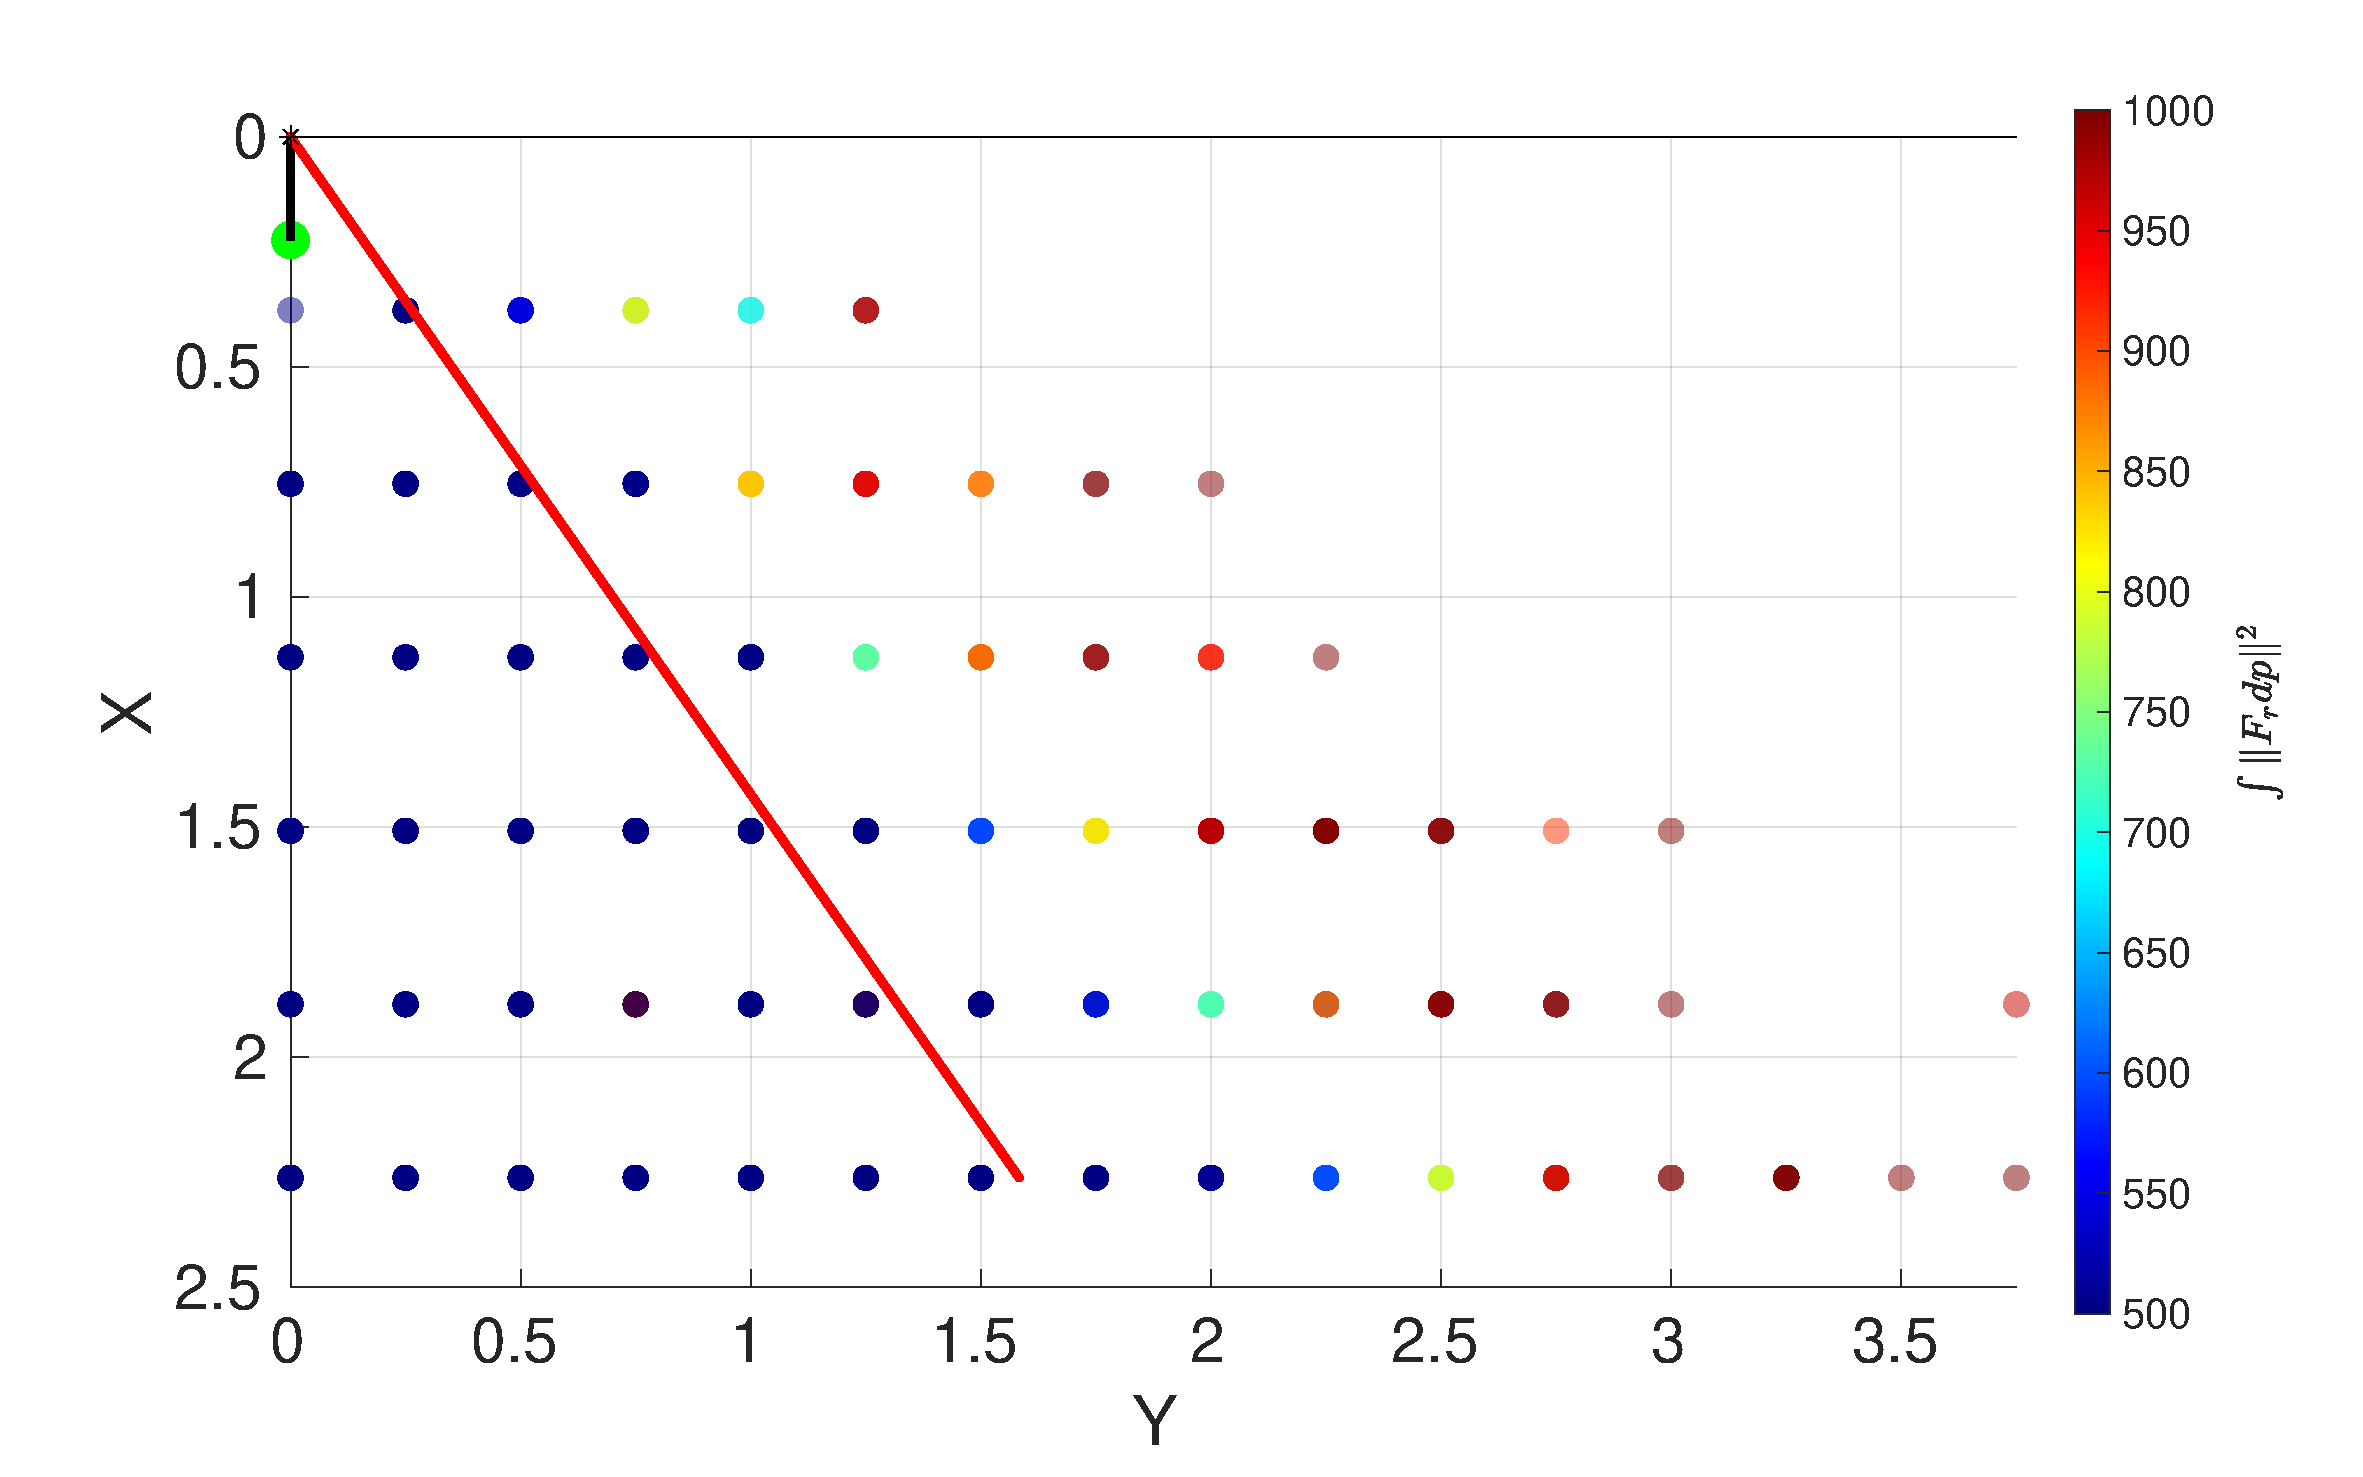
\includegraphics[width=\columnwidth]{matlab/reachable.pdf}
	\caption{\small Simulation. Plot of the region of reachable targets for a friction coefficient $\mu =0.7$.}
	\label{fig:reachable_region}
\end{figure}
